\documentclass[conference]{IEEEtran}
\IEEEoverridecommandlockouts
\usepackage{cite}
\usepackage{amsmath,amssymb,amsfonts}
\usepackage{graphicx}
\usepackage{textcomp}
\usepackage{xcolor}
\usepackage{xurl}
\usepackage{booktabs}
\usepackage[hidelinks]{hyperref}
\urlstyle{tt}

\def\BibTeX{{\rm B\kern-.05em{\sc i\kern-.025em b}\kern-.08em
    T\kern-.1667em\lower.7ex\hbox{E}\kern-.125emX}}

\begin{document}

\title{Throughput and Acceleration Trade-offs of Lightweight Block Ciphers:\\
A CPU and GPU Comparison of PRESENT-80, SPECK-64/128, and AES-128}

\author{%
  \hfill\begin{minipage}[t]{0.30\textwidth}
    \centering
    Devansh Gupta\\
    \textit{Dept. of Electrical and Computer Engineering}\\
    University of California San Diego\\
    San Diego, CA, USA\\
    d6gupta@ucsd.edu
  \end{minipage}\hfill%
  \begin{minipage}[t]{0.30\textwidth}
    \centering
    Priyansh Parikh\\
    \textit{Dept. of Electrical and Computer Engineering}\\
    University of California San Diego\\
    San Diego, CA, USA\\
    p2parikh@ucsd.edu
  \end{minipage}\hfill%
  \begin{minipage}[t]{0.30\textwidth}
    \centering
    Jeevan N V\\
    \textit{Dept. of Electrical and Computer Engineering}\\
    University of California San Diego\\
    San Diego, CA, USA\\
    jnv@ucsd.edu
  \end{minipage}\hfill%
}

\maketitle

\begin{abstract}
Lightweight block ciphers are designed to fit within the stringent silicon area budgets of constrained
IoT hardware where standards like AES-128 are too heavy. However, the software and GPU throughput
characteristics of these architectural families are rarely compared against AES on a single, controlled
platform. This paper presents from-scratch C++ and CUDA implementations of PRESENT-80, SPECK-64/128,
and AES-128, validated against official test vectors and benchmarked on an AMD EPYC CPU and an NVIDIA
L40S GPU. Our evaluation shows that the Add-Rotate-XOR (ARX) design of SPECK achieves massive
performance advantages, leading CPU and GPU encryption throughput at 1,133~MB/s and 356~GB/s,
respectively, while minimizing key-schedule latency and device memory footprint. Conversely, the
Substitution-Permutation Network (SPN) design of PRESENT-80 yields the lowest absolute throughput but
achieves the highest relative GPU speedup (over 5,200$\times$) by mitigating severe CPU-side
bit-manipulation inefficiencies. Furthermore, we identify a 37\% performance drop specific to AES-128
in Counter (CTR) mode on the GPU, driven by per-thread register pressure inherent to its
table-intensive structure. These insights demonstrate that ARX ciphers uniquely align hardware area
constraints with software and parallel processing scalability, providing critical design guidance for
secure IoT ecosystems.
\end{abstract}

\begin{IEEEkeywords}
lightweight cryptography, block cipher, PRESENT, SPECK, AES, GPU, CUDA, IoT security, throughput
\end{IEEEkeywords}

\section{Introduction}

The proliferation of IoT devices has created demand for encryption that operates within tight resource
budgets. The smallest constrained targets, including passive RFID tags, medical implants, and sensor
nodes, impose silicon area budgets near 2,000 gate equivalents (GE), memory as small as a few hundred
bytes, and power budgets measured in microwatts~\cite{survey}. AES-128 requires approximately 3,400 GE
in hardware~\cite{fips197}, which exceeds the IoT budget and motivates dedicated lightweight cipher
design.

Two prominent design families have emerged. Substitution-Permutation Network (SPN) ciphers, exemplified
by PRESENT-80~\cite{present}, use structured S-box substitution and bit-permutation rounds. Their
permutation layers are wire-routing in dedicated silicon and cost essentially nothing in hardware area,
but become explicit bit-manipulation operations in software. Add-Rotate-XOR (ARX) ciphers, exemplified
by SPECK-64/128~\cite{speck}, use only modular addition, rotation, and XOR per round. These operations
map directly to native CPU and GPU integer arithmetic units with no table lookups, making ARX designs
fast in software while remaining compact in hardware.

Prior work reports hardware GE footprints for these ciphers in isolation. A direct platform-controlled
comparison of CPU throughput, GPU throughput, key-schedule cost, and mode behavior on modern server
hardware has not been published for these specific cipher families. This paper fills that gap with a
consistent implementation and measurement methodology.

The contributions of this work are as follows. We implement all three ciphers from scratch in C++ and
CUDA without any third-party cryptographic libraries, hardware intrinsics, or vendor-optimized paths,
and validate each against its official reference vectors. We measure ECB, CTR, and CBC CPU throughput
across five buffer sizes spanning 1~KB to 64~MB. We characterize GPU ECB and CTR throughput on an
NVIDIA L40S and derive speedup ratios relative to the CPU baseline. We measure key-schedule latency
and device memory footprint per cipher. We analyze the resulting trade-off between hardware area,
software throughput, GPU scalability, and standardization coverage.

The remainder of this paper is organized as follows. Section~II provides background on cipher
construction and hardware footprint. Section~III describes the implementation. Section~IV describes
the experimental setup. Section~V presents results. Section~VI discusses the implications.
Section~VII concludes.

\section{Background}

\subsection{Cipher Constructions}

An SPN cipher alternates substitution and permutation layers in each round. Substitution provides
nonlinearity through S-box lookups and permutation diffuses S-box outputs across the full state.
PRESENT-80 uses a 4-bit S-box and a deterministic bit permutation that maps bit position $j$ to
position $(16j) \bmod 63$. AES-128 uses an 8-bit S-box, ShiftRows, MixColumns over
GF$(2^8)$, and AddRoundKey. The AES S-box and its inverse together occupy 512 bytes of device
constant memory in the GPU implementation.

An ARX cipher applies one round of modular addition, word rotation, and XOR. SPECK-64/128 computes
$x \leftarrow (\mathrm{ROR}(x, 8) + y) \oplus k$ and $y \leftarrow \mathrm{ROL}(y, 3) \oplus x$ per
round. This requires no lookup tables, so SPECK's GPU device footprint consists entirely of round keys.

Table~\ref{tab:specs} summarizes the cipher parameters.

\begin{table}[t]
\caption{Cipher Specifications}
\label{tab:specs}
\begin{center}
\begin{tabular}{|l|c|c|c|c|}
\hline
\textbf{Cipher} & \textbf{Type} & \textbf{Block} & \textbf{Key} & \textbf{Rounds} \\
\hline
PRESENT-80     & SPN & 64-bit  & 80-bit  & 31 \\
SPECK-64/128   & ARX & 64-bit  & 128-bit & 27 \\
AES-128        & SPN & 128-bit & 128-bit & 10 \\
\hline
\end{tabular}
\end{center}
\end{table}

\subsection{Hardware Area Footprint}

Table~\ref{tab:ge} lists published hardware area estimates for each cipher. SPECK-64/128 and
PRESENT-80 both fit within the 2,000~GE IoT area budget. AES-128 does not.

\begin{table}[t]
\caption{Published Hardware Area Estimates}
\label{tab:ge}
\begin{center}
\begin{tabular}{|l|c|c|}
\hline
\textbf{Cipher} & \textbf{Area (GE)} & \textbf{Fits $<$2,000 GE} \\
\hline
PRESENT-80    & $\approx$1,570~\cite{present} & Yes \\
SPECK-64/128  & $\approx$1,280~\cite{speck}   & Yes \\
AES-128       & $\approx$3,400~\cite{fips197}  & No  \\
\hline
\end{tabular}
\end{center}
\end{table}

\subsection{Modes of Operation}

ECB (Electronic Codebook) encrypts each block independently and serves as the primary throughput
benchmark mode in this work~\cite{sp80038a}. CTR (Counter mode) encrypts successive counter values
and XORs each result with the corresponding plaintext block, making all blocks fully independent
and suitable for parallel GPU execution. CBC (Cipher-Block Chaining) XORs each plaintext block
with the previous ciphertext before encryption, making forward encryption sequential while
allowing parallel decryption.

\section{Implementation}

\subsection{CPU Implementation}

All three ciphers are implemented in C++17 and compiled with \texttt{g++ 13.3 -O3}. The host interface
follows a uniform batch API in which a caller provides a key, plaintext buffer, and block count.
PRESENT-80 and SPECK-64/128 share this interface and are validated against the official CHES~2007
and NSA~2013 reference vectors, respectively. AES-128 is validated against FIPS-197 Appendix~B and
Appendix~C test vectors. SPECK-64/128 decryption was explicitly optimized for CPU to reduce per-block
cycle count relative to a direct inverse of the encryption schedule.

\subsection{GPU Implementation}

All CUDA kernels are compiled with \texttt{nvcc -O3} targeting CUDA~12.8~\cite{cuda}. Each kernel launches one
thread per cipher block, which allows the GPU scheduler to assign independent AES, SPECK, or PRESENT
rounds to threads without any synchronization.

Round keys are computed entirely on the CPU host and uploaded to device constant memory via
\texttt{cudaMemcpyToSymbol}. Constant memory is a read-only GPU address space that is cached and
broadcast to all threads in a warp at zero per-thread cost. Key-schedule time is excluded from all
GPU kernel measurements because a single schedule is amortized over all blocks processed under one
key. ECB and CTR kernels are provided for all three ciphers. The CTR kernel constructs an independent
counter per thread from the block index and XORs the encrypted counter with the corresponding
plaintext block.

Table~\ref{tab:ks} lists the device constant memory breakdown per cipher. SPECK-64/128 requires no
S-box and occupies only 108 bytes. AES-128 stores forward and inverse S-boxes (256 bytes each) plus
round keys (176 bytes) for a total of 688 bytes in ECB mode, and 432 bytes in CTR mode because CTR
requires only the forward S-box. PRESENT-80 stores 256 bytes of round keys and 32 bytes for its
compact 4-bit S-box pair (288 bytes total for ECB, 272 bytes for CTR with only the forward S-box).

\begin{table}[t]
\caption{Key Schedule and Device Constant Memory Footprint}
\label{tab:ks}
\begin{center}
\begin{tabular}{|l|c|c|c|c|c|}
\hline
\textbf{Cipher} & \textbf{RK (B)} & \textbf{S-box (B)} & \textbf{Total (B)} & \textbf{KS ($\mu$s)} & \textbf{KS cyc} \\
\hline
PRESENT-80    & 256 & 32  & 288 & 2.20  & 8,465 \\
SPECK-64/128  & 108 & 0   & 108 & 0.026 & 100   \\
AES-128       & 176 & 512 & 688 & 0.094 & 360   \\
\hline
\end{tabular}
\end{center}
\end{table}

\subsection{Correctness Validation}

All six mode roundtrip tests (ECB, CTR, and CBC for each cipher) across the CPU implementations
pass complete encrypt-decrypt verification. For the GPU, CBC mode was not implemented due to its
inherent block-to-block data dependencies, which prevent parallelization and conflict with the GPU's
multi-threaded execution model. No timing data is recorded unless the corresponding validation check
passes.

\section{Experimental Setup}

All experiments run on an AMD EPYC 9374F 32-core processor paired with an NVIDIA L40S GPU~\cite{l40s}.
Each measurement is the mean of five independent trials. Buffer sizes sweep from 1~KB to 64~MB in
five steps (1~KB, 64~KB, 1~MB, 16~MB, 64~MB), spanning a 65,536-fold range of input volume to
characterize small-buffer overhead and large-buffer steady-state throughput separately.

GPU measurements record kernel execution time only, excluding host-to-device data transfer.
CPU measurements use the \texttt{RDTSC} hardware timestamp counter for cycle-accurate timing.
All benchmarks run in ECB mode unless otherwise noted. Mode-overhead measurements (CTR and CBC)
use fixed 1~MB payloads for the CPU and the full sweep for GPU CTR.

\section{Results}

\subsection{CPU Throughput}

Table~\ref{tab:cpu} shows CPU ECB encryption and decryption throughput. SPECK-64/128 sustains
approximately 1,133~MB/s for encryption at all buffer sizes, which is 47 times faster than AES-128 at
23.87~MB/s and 784 times faster than PRESENT-80 at 1.4451~MB/s at 64~MB. Throughput is nearly flat
across buffer size for all three ciphers, indicating that each workload is compute-bound with the
cipher state resident in processor cache.

AES-128 decryption is considerably slower than encryption at approximately 15.0~MB/s across all
buffer sizes, because the inverse cipher path requires additional table accesses that have no hardware
equivalent at this optimization level. PRESENT-80 is nearly symmetric, reaching 1.4270~MB/s in
decryption at 64~MB. SPECK-64/128 decryption is somewhat slower than encryption, at 850.54~MB/s
versus 1,132.77~MB/s at 64~MB, reflecting the sequential inverse key-schedule traversal required
per block.

The per-block cost explains the throughput ordering directly. SPECK-64/128 requires 39 cycles per
block and 3.10 cycles per byte. AES-128 requires 2,580 cycles per block and 161 cycles per byte.
PRESENT-80 requires 21,136 cycles per block and 734 cycles per byte, as shown in
Table~\ref{tab:latency}.

\begin{table*}[t]
\caption{CPU ECB Throughput (MB/s): Encryption and Decryption}
\label{tab:cpu}
\begin{center}
\begin{tabular}{|l|c|c|c|c|c|c|}
\hline
\textbf{Size} & \textbf{PRESENT enc} & \textbf{PRESENT dec} & \textbf{SPECK enc}
  & \textbf{SPECK dec} & \textbf{AES enc} & \textbf{AES dec} \\
\hline
1~KB  & 1.4791 & 1.4662 & 1167.73 & 880.24 & 23.80 & 15.02 \\
64~KB & 1.4448 & 1.4255 & 1225.82 & 899.78 & 23.88 & 15.04 \\
1~MB  & 1.4456 & 1.4282 & 1098.32 & 849.03 & 23.85 & 15.04 \\
16~MB & 1.4453 & 1.4272 & 1131.34 & 844.62 & 23.84 & 14.99 \\
64~MB & 1.4451 & 1.4270 & 1132.77 & 850.54 & 23.87 & 15.02 \\
\hline
\end{tabular}
\end{center}
\end{table*}

\begin{table}[t]
\caption{Single-Block CPU Cost}
\label{tab:latency}
\begin{center}
\begin{tabular}{|l|c|c|c|}
\hline
\textbf{Cipher} & \textbf{cyc/byte} & \textbf{Block cycles} & \textbf{Latency ($\mu$s)} \\
\hline
PRESENT-80    & 734  & 21,136 & $\approx$5.0   \\
SPECK-64/128  & 3.10 & 39     & $\approx$0.009 \\
AES-128       & 161  & 2,580  & $\approx$0.62  \\
\hline
\end{tabular}
\end{center}
\end{table}

\subsection{GPU ECB Throughput and Speedup}

At 64~MB, SPECK-64/128 reaches 356,150~MB/s in ECB encryption, AES-128 reaches 32,672~MB/s, and
PRESENT-80 reaches 7,519~MB/s. At 1~KB, all three ciphers underperform (SPECK 571.7, AES 88.9,
PRESENT 43.9~MB/s) because the buffer holds too few blocks to saturate the L40S. Throughput rises
sharply between 64~KB and 1~MB as GPU parallelism fills the device, and stabilizes above 16~MB.

SPECK-64/128 shows an elevated peak at 16~MB of 823,317~MB/s in ECB encryption, 2.3 times its
64~MB value. This behavior is discussed in Section~\ref{sec:disc}.

GPU speedup over the CPU ECB baseline at 64~MB is approximately 5,203 times for PRESENT-80, 1,370
times for AES-128, and 314 times for SPECK-64/128. The speedup ordering inverts the absolute
throughput ordering: the cipher with the weakest CPU performance (PRESENT-80) gains the largest
relative multiplier. Fig.~\ref{fig:speck} shows the full throughput and speedup scaling curves for SPECK-64/128.
Fig.~\ref{fig:present} and Fig.~\ref{fig:aes} show the corresponding curves for PRESENT-80
and AES-128.

\subsection{GPU CTR Mode Performance}

Table~\ref{tab:gpu} reports GPU peak throughput at 64~MB for ECB and CTR modes. PRESENT-80 and
SPECK-64/128 show negligible difference between modes. SPECK-64/128 ECB encryption is 356,150~MB/s
and CTR is 357,693~MB/s, a difference below 0.5 percent. PRESENT-80 shows 7,519 versus 7,502~MB/s,
within 0.2 percent.

AES-128 behaves differently. Its CTR encryption is 20,626~MB/s at 64~MB, which is 37 percent below
its ECB value of 32,672~MB/s. The same gap appears at 1~MB (CTR 17,536 versus ECB 26,580~MB/s) and
16~MB (CTR 20,554 versus ECB 32,461~MB/s). The cause is analyzed in Section~\ref{sec:disc}.

\begin{table*}[t]
\caption{GPU Peak Throughput at 64~MB (MB/s): ECB and CTR, Encryption and Decryption}
\label{tab:gpu}
\begin{center}
\begin{tabular}{|l|c|c|c|c|c|}
\hline
\textbf{Cipher} & \textbf{ECB enc} & \textbf{ECB dec}
  & \textbf{CTR enc} & \textbf{CTR dec} & \textbf{Speedup vs CPU (ECB enc)} \\
\hline
PRESENT-80    & 7,518.84    & 7,509.61    & 7,501.53    & 7,502.71    & $\approx$5,203$\times$ \\
SPECK-64/128  & 356,149.73  & 486,307.40  & 357,692.65  & 482,192.59  & $\approx$314$\times$   \\
AES-128       & 32,671.82   & 35,436.36   & 20,626.12   & 20,638.33   & $\approx$1,370$\times$ \\
\hline
\end{tabular}
\end{center}
\end{table*}

\subsection{Key Schedule Analysis}

PRESENT-80 is the most expensive cipher to initialize at 2.20~$\mu$s and 8,465 cycles, approximately
85 times slower than SPECK-64/128 (100 cycles) and 23.5 times slower than AES-128 (360 cycles). The
high PRESENT-80 cost reflects its 31-round key extraction from an 80-bit key register. SPECK-64/128
has the smallest device footprint at 108 bytes, compared to 288 bytes for PRESENT-80 and 688 bytes
for AES-128 in ECB mode. Notably, the AES-128 S-box tables alone (512 bytes) exceed the entire
SPECK-64/128 device footprint. See Table~\ref{tab:ks} in Section~III.

\subsection{Mode Overhead on CPU}

Table~\ref{tab:modes} shows CPU throughput for ECB, CTR, and CBC. AES-128 changes little across
modes: ECB 23.6, CTR 21.56, CBC 22.08~MB/s. The cipher is slow enough that per-block mode
bookkeeping is a negligible fraction of total work. SPECK-64/128 shows the largest relative penalty:
CTR drops 53 percent from ECB (528.7 versus 1,133~MB/s) and CBC drops 74 percent (291.0~MB/s). A
fast cipher makes per-block counter increments and sequential CBC chaining costs visible. PRESENT-80
shows little change across modes in relative terms (ECB 1.45, CTR 1.40, CBC 1.33~MB/s) because
round computation dominates all other overhead.

\begin{table}[t]
\caption{CPU Throughput by Mode of Operation (MB/s)}
\label{tab:modes}
\begin{center}
\begin{tabular}{|l|c|c|c|}
\hline
\textbf{Cipher} & \textbf{ECB} & \textbf{CTR} & \textbf{CBC} \\
\hline
PRESENT-80    & $\approx$1.45  & 1.40  & 1.33  \\
SPECK-64/128  & $\approx$1,133 & 528.7 & 291.0 \\
AES-128       & $\approx$23.6  & 21.56 & 22.08 \\
\hline
\end{tabular}
\end{center}
\end{table}

\begin{figure*}[t]
\centerline{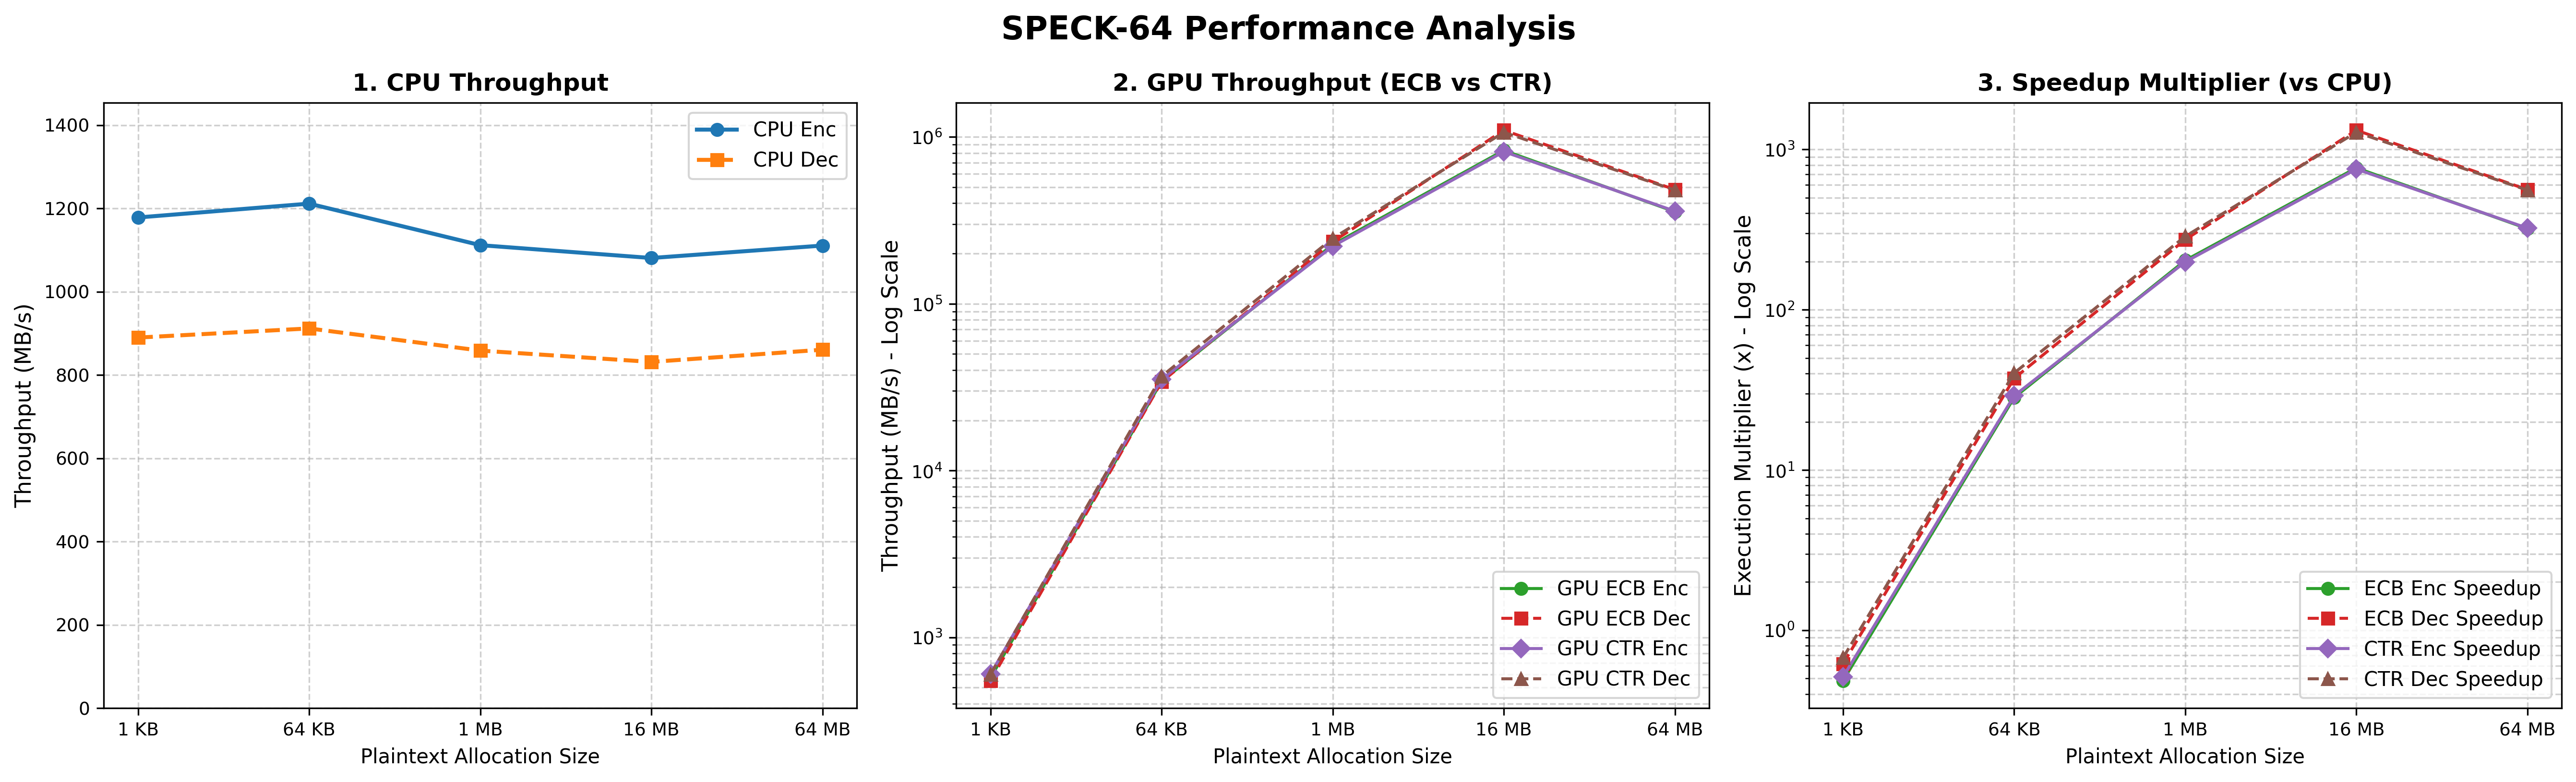
\includegraphics[width=\textwidth]{../run_outputs/speck64_performance_graphs.png}}
\caption{SPECK-64/128 performance. Panel 1: CPU ECB throughput (linear scale). Panel 2: GPU ECB
and CTR throughput (log scale). Panel 3: GPU speedup over CPU baseline (log scale).}
\label{fig:speck}
\end{figure*}

\begin{figure*}[t]
\centerline{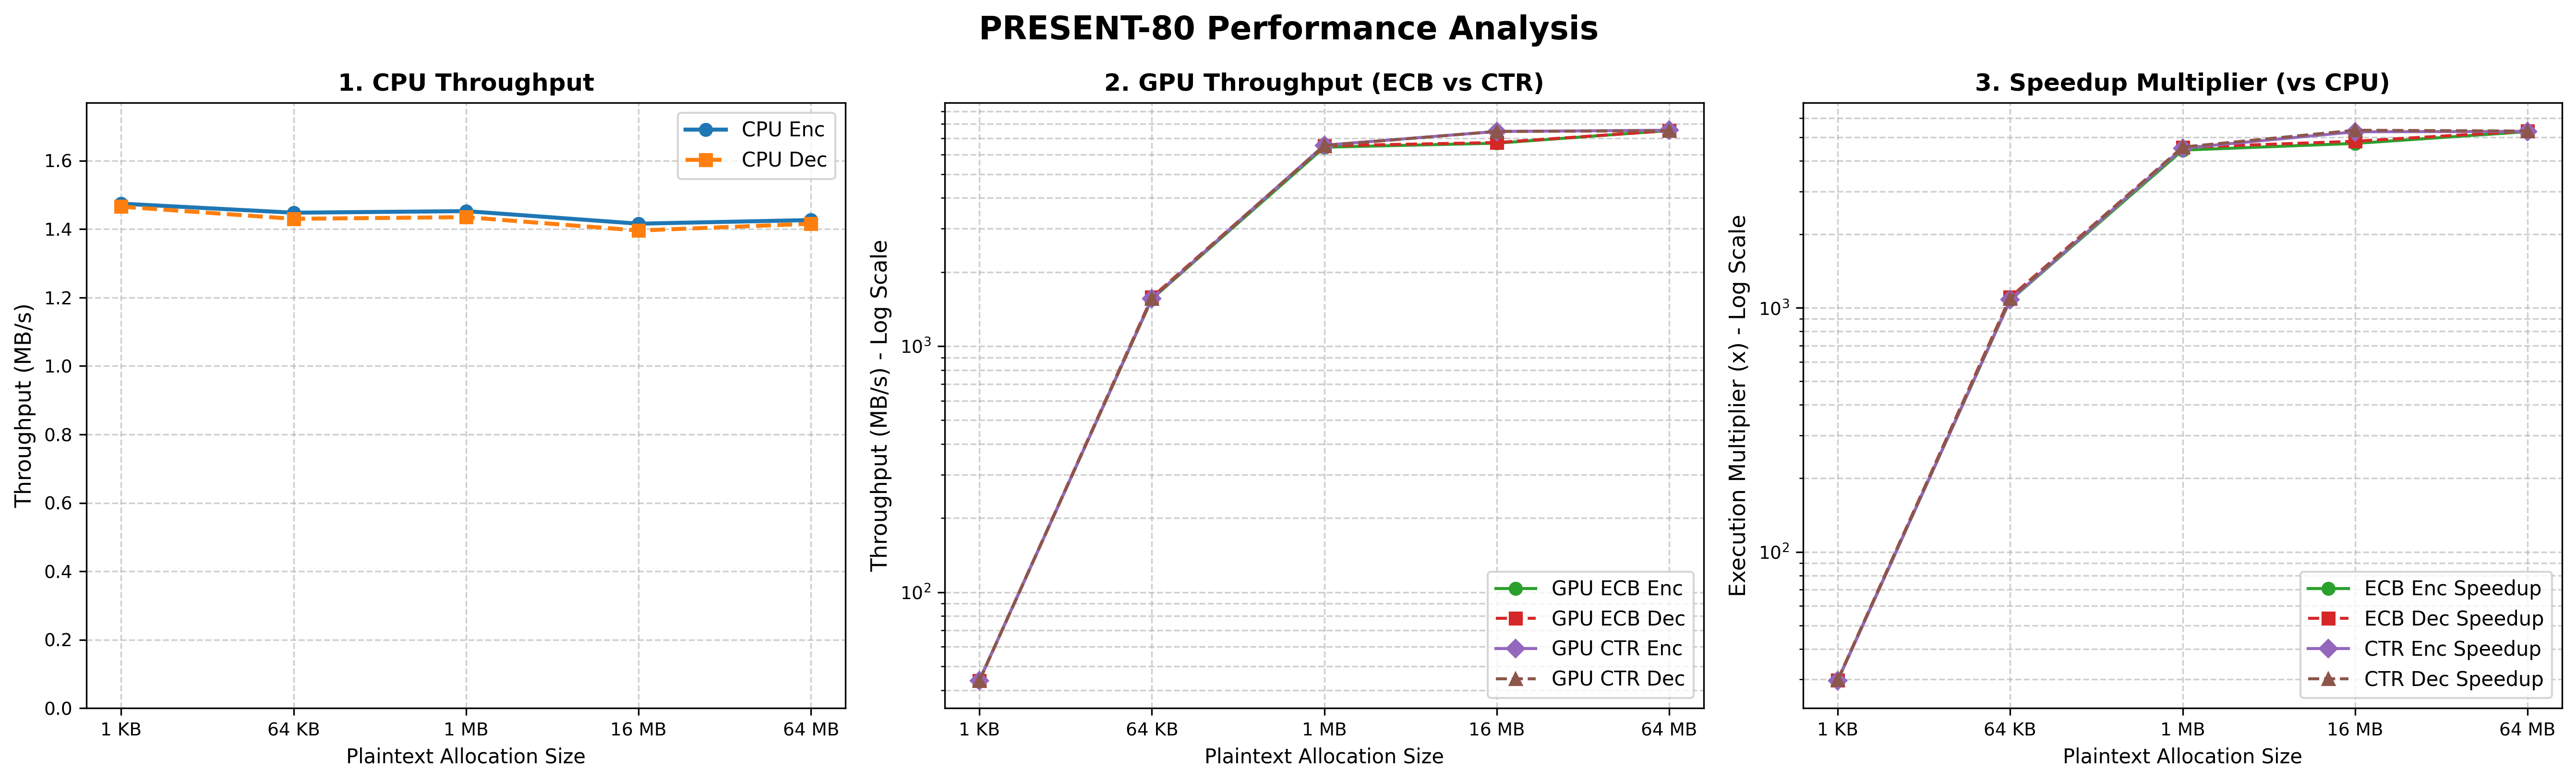
\includegraphics[width=\textwidth]{../run_outputs/present80_performance_graphs.png}}
\caption{PRESENT-80 performance. Panel 1: CPU ECB throughput (linear scale). Panel 2: GPU ECB
and CTR throughput (log scale). Panel 3: GPU speedup over CPU baseline (log scale).}
\label{fig:present}
\end{figure*}

\begin{figure*}[t]
\centerline{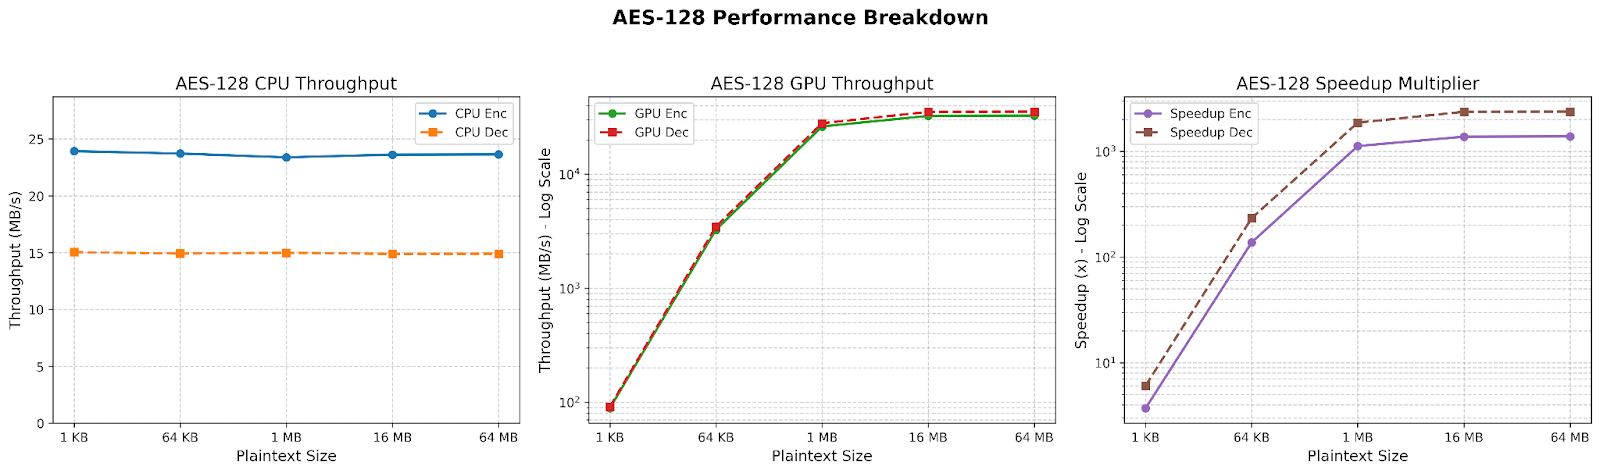
\includegraphics[width=\textwidth]{../run_outputs/aes128_performance_graphs_corrected.png}}
\caption{AES-128 performance. Panel 1: CPU ECB throughput (linear scale). Panel 2: GPU ECB
and CTR throughput (log scale). Panel 3: GPU speedup over CPU baseline (log scale).}
\label{fig:aes}
\end{figure*}

\section{Discussion}
\label{sec:disc}

\textbf{Largest speedup versus lowest absolute throughput.} PRESENT-80 achieves a 5,203-times GPU
speedup despite sustaining only 1.445~MB/s on the CPU, the largest relative gain in this study. The
GPU hides per-thread latency by executing thousands of independent blocks concurrently, so the
relative gain is largest precisely where the CPU baseline is weakest. This is a symptom of CPU
inefficiency, not of intrinsic GPU friendliness. In absolute terms, PRESENT-80 still trails
SPECK-64/128 on the GPU by approximately 47 times (7,519 versus 356,150~MB/s). A high speedup ratio
alone does not indicate high absolute performance.

\textbf{ARX aligns area and throughput.} SPECK-64/128 achieves the smallest hardware footprint
($\approx$1,280~GE), the smallest device constant memory (108~bytes), and the highest CPU and GPU
throughput among the three ciphers. These properties are not coincidental. ARX operations map
directly to native integer ALUs with no table lookups and no dedicated S-box combinational logic.
The same absence of S-box hardware that keeps silicon area small also eliminates memory bandwidth
and instruction overhead in software. SPN ciphers do not share this alignment. The bit permutation
that is cost-free in hardware (a set of wires) becomes explicit bit-manipulation in software, and
the S-box that is compact in silicon requires memory access in software. SPECK demonstrates that a
cipher can jointly minimize area and maximize throughput when the design avoids table-based
operations entirely.

\textbf{AES CTR throughput drop on GPU.} The 37-percent gap between AES-128 ECB and CTR GPU
throughput (32,672 versus 20,626~MB/s at 64~MB) does not appear in PRESENT-80 or SPECK-64/128,
and warrants explanation. The AES CTR kernel uses only the forward S-box and requires 432 bytes of
constant memory, less than the 688 bytes used by the ECB kernel. Lower constant memory usage
should, in isolation, improve cache efficiency. The observed degradation therefore points to
per-thread register pressure rather than constant cache capacity as the root cause. Constructing a
128-bit counter and feeding it through ten AES rounds requires more registers per thread than the
direct plaintext path in ECB mode, reducing warp occupancy on the L40S. SPECK-64/128 and
PRESENT-80 have sufficient register headroom for CTR's counter construction at their respective
round counts (27 and 31 rounds) and show no occupancy reduction. This finding suggests that the
CTR mode penalty for AES is specific to table-intensive SPN kernels with high per-thread state
requirements.

\textbf{SPECK-64/128 throughput at 16~MB versus 64~MB.} SPECK-64/128 ECB encryption peaks at
823,317~MB/s at 16~MB then settles to 356,150~MB/s at 64~MB. At 16~MB the working set interacts
favorably with the L40S GPU L2 cache and the kernel is compute-bound throughout execution. At 64~MB
the buffer exceeds effective L2 capacity, the kernel transitions to a memory-bandwidth-limited
regime, and throughput is bounded by the device memory bus rather than by the cipher's arithmetic
rate. We report the 64~MB value as the stable steady-state throughput for SPECK-64/128.

\textbf{System design implications.} For constrained devices where AES compliance is not mandated,
SPECK-64/128 is the strongest choice across all software and GPU metrics, fitting within the
2,000~GE area budget while leading in throughput. PRESENT-80 is appropriate when ISO/IEC 29192-2
compliance~\cite{iso29192} or a purely hardware-oriented SPN structure is required, with the understanding that
its software throughput is poor by design. AES-128 is correct when FIPS-197 compliance is
mandatory. Its CPU performance of 23.87~MB/s in this study uses no AES-NI instructions, so
hardware-accelerated deployments would substantially exceed this baseline. The central conclusion
is that hardware area, software throughput, GPU scalability, and cryptographic standardization
rarely optimize together, and ARX ciphers such as SPECK come closest to satisfying the first
three simultaneously.

\section{Conclusion}

This paper presents from-scratch C++ and CUDA implementations of PRESENT-80, SPECK-64/128, and
AES-128, validated against official test vectors and benchmarked on an AMD EPYC 9374F CPU and
NVIDIA L40S GPU. SPECK-64/128 leads all three ciphers in CPU encryption throughput (1,133~MB/s),
GPU peak throughput (356,150~MB/s), key-schedule speed (100 cycles), and device footprint (108 bytes).
PRESENT-80 achieves the largest GPU speedup at 5,203 times over its CPU baseline but the lowest
absolute throughput in every configuration. AES-128 delivers the broadest standardization coverage
and requires hardware AES instructions to be competitive on CPU throughput. Counter mode GPU
throughput matches ECB for PRESENT-80 and SPECK-64/128 but falls 37 percent for AES-128, identifying
a register-pressure effect tied to the AES table-intensive SPN kernel. Future work includes
incorporating AES-NI for a fair modern comparison, porting to microcontroller-class targets,
measuring end-to-end GPU latency including host-device transfer, and evaluating ASCON as the NIST
Lightweight Cryptography competition winner.

\section*{Source Code}
\noindent\raggedright
The full source code and benchmark logs are publicly available at\\[2pt]
\href{https://github.com/devansh-gupta19/ECE268-Lightweight_block_cipher}{%
\small\texttt{https://github.com/devansh-gupta19/}}\\[1pt]
\href{https://github.com/devansh-gupta19/ECE268-Lightweight_block_cipher}{%
\small\texttt{ECE268-Lightweight\_block\_cipher}}\par

\begin{thebibliography}{00}

\bibitem{present}
A. Bogdanov, L. R. Knudsen, G. Leander, C. Paar, A. Poschmann, M. J. B. Robshaw, Y. Seurin, and
C. Vikkelsoe, ``PRESENT: An ultra-lightweight block cipher,'' in \textit{Proc. Int. Workshop
Cryptographic Hardware and Embedded Systems (CHES)}, Vienna, Austria, Sept. 2007, pp. 450--466.

\bibitem{speck}
R. Beaulieu, D. Shors, J. Smith, S. Treatman-Clark, B. Weeks, and L. Wingers, ``The SIMON and
SPECK families of lightweight block ciphers,'' Cryptology ePrint Archive, Report 2013/404,
National Security Agency, Fort Meade, MD, USA, 2013.

\bibitem{fips197}
National Institute of Standards and Technology, ``Federal Information Processing Standard (FIPS)
197: Advanced Encryption Standard (AES),'' NIST FIPS~197, Nov. 2001.

\bibitem{iso29192}
International Organization for Standardization, ``ISO/IEC 29192-2:2019 -- Information Security --
Lightweight Cryptography -- Part 2: Block Ciphers,'' Geneva, Switzerland, 2019.

\bibitem{sp80038a}
E. Barker and M. Smid, ``Recommendation for Block Cipher Modes of Operation: Methods and
Techniques,'' NIST Special Publication 800-38A, Dec. 2001.

\bibitem{cuda}
NVIDIA Corporation, ``CUDA C++ Programming Guide,'' Version 12.8, 2024.
[Online]. Available: \url{https://docs.nvidia.com/cuda/cuda-c-programming-guide/}

\bibitem{survey}
A. Poschmann, ``Lightweight Cryptography: Cryptographic Engineering for a Pervasive World,''
Ph.D. dissertation, Ruhr University Bochum, Germany, 2009.

\bibitem{l40s}
NVIDIA Corporation, ``NVIDIA L40S PCIe GPU -- Technical Specifications,'' 2023.
[Online]. Available: \url{https://www.nvidia.com/en-us/data-center/l40s/}

\end{thebibliography}

\end{document}
